\section{Elettroni nel potenziale periodico}
Un materiale solido \`e possibile rappresentarlo come un reticolo, di una sua certa complessit\`a, che si ripete nello spazio in modo periodico. Il fatto che il reticolo di un cristallo, per definizione, sia dotato di una periodicit\`a spaziale permette di associarci in modo naturale la sua rappresentazione di Fourier nello spazio dei vettori d'onda $\xv{k} $. I metalli sono caratterizzati dall'avere orbitali atomici fortemente interagenti creando forti legami ti di tipo \textit{Tight Binding}. Questa caratteristica, unita al fatto che la temperatura di Fermi di un metallo \`e solitamente molto alta rispetto alla temperatura ambiente, permette di pensare la dinamica degli elettroni, in un metallo, come la dinamica di un gas libero di elettroni, all'interno di un potenziale periodico.

Il problema degli elettroni liberi in un potenziale periodico si riduce al seguente problema agli autovalori
\newl{\left[-\frac{\hbar^2}{2m}\nabla^2_r +U_e(\xv{r} )\right]\psi_n(\xv{r} ) = E_n \psi_n(\xv{r} ),}
con le seguenti assunzioni:
\begin{itemize}
	\item Elettroni \textbf{indipendenti}: In questo modo la funzoine d'onda che descrive il problema è possibile fattorizzarla;
	\item Il potenziale è \textbf{periodico}: Questo vuol dire che $U(\xv{r}  + \xv{R} )  = U(\xv{r}  )$.
\end{itemize}
Il teorema di Bloch afferma che per un potenziale periodico la funzoine d'onda è possibile fattorizzarla in una parte di onda piana e in una parte periodica
\newl{\boxed{\psi_{n,\xv{k} }(\xv{r} )=\overbracket{e^{i\xv{k} \cdot\xv{r} }}^{\text{Onda Piana}} \overbracket{u_{n,\xv{k} }(\xv{r} ) }^{\text{Periodica}}}}

\subsection{Giustificazione fisica del teorema di Bloch}
La giustificazione del teorema di Bloch e quindi della forma delle funzioni d'onda dell'elettrone libero all'interno di un cristallo, trova la sua base sulle ipotesi fatte appunto sul reticolo cristallino stesso. Il reticolo cristallino gode di periodicit\`a spaziale quindi ci si aspetta che i moduli quadri della funzione d'onda siano periodici con periodo uguale al passo del reticolo cristallino
\newl{\abs{\psi(\xv{r} )} ^2 = \abs{\psi(\xv{r} +\xv{R} )} ^2.}
La funzione d'onda avrà una sua parte radiale con un certo coefficiente $C_{\vet k}$, per il quale deve valere che $\abs{C_k} =1$. Un modo diretto per visualizzare questa condizione consiste nel pensare il coefficiente $C_{\vet k}$ come un'onda piana e successivamente cercare l'ugualianza tra le parti radiali di $\psi_k(\xv{r} )$ r $\psi_k(\xv{r} +\xv{R} )$, notiamo che:
\newl{e^{i\xv{k} \cdot \xv{r} }\left[e^{-i\xv{k} \cdot \xv{r} } u_{n,\xv{k} }(\xv{r} )\right] = e^{i\xv{k} \cdot \xv{r} }e^{i\xv{k} \cdot \xv{R} } \left[ e^{-i\xv{k} \cdot \xv{r} }e^{-i\xv{k} \cdot \xv{R} }u_{n,\xv{k} }(\xv{r} +\xv{R} )\right]}
da cui
\newl{\boxed{u_{n,\xv{k} }(\xv{r} ) = u_{n,\xv{k} }(\xv{r} + \xv{R} ) }.}
In questo modo si vuole dare una giustificazione molto intuitiva del perchè le funzioni d'onda del teorema di Bloch sono funzioni d'onda sensate che seguono bene le condizioni di periodicità del nostro problema. Le soluzioni dell'Hamiltoniana sono in funzione alle condizioni al bordo che scegliamo. In questo caso, data la simmetria del problema, \`e opportuno scegliere delle condizioni al bordo periodiche. La restrizione sui valori di $\xv{k} $ sarà data da una serie di considerazioni. Partendo dalla periodicità della funzione d'onda $\psi(\xv{r} ) = \psi(\xv{r} +\xv{L} )$ sul reticolo, se $\xv{a} $ è un vettore del reticolo diretto si ha che $L = Na$. Uguagliando le funzioni d'onda
\newl{e^{i\xv{k} \cdot \xv{x} } = e^{i\xv{k} \cdot (\xv{x} + \xv{L} )} u_{\xv{k} }(\xv{x} +\xv{L} )} 
prendendo in considerazione solo i moduli, si giunge alla nota condizione
\newl{\boxed{kL = n 2\pi\implicaa k=\frac{2\pi}{L}n\,\,\, \text{ dove } \,\,\,n\in\Z .}}
Questa appena scritta è la famosa condizione periodica di \textit{\textbf{Born - Von Karman}}. Dal punto di vista dello spazio dei vettori $\vet k$, questo ci dice che le funzioni d'onda possono essere tutte rimappate nell'intervallo di $k\in\left[-\frac{\pi}{a},\frac{\pi}{a}\right]$. Zona nota come \textit{Prima Zona di Brillouin}. Nello spazio $\xv{k} $ posso verificare facilmente che $\xv{k}  = \xv{k} '-\xv{G} $ dove $\xv{G} $ è un vettore di base del reticolo reciproco
\newl{\psi_{\xv{k} '}(\xv{x} )e^{i\xv{k} ' \cdot \xv{x} }u_{\xv{k} '}(\xv{x} ) = e^{i(\xv{k} + \xv{G} )\cdot \xv{x} }u_{\xv{k} +\xv{G} }(\xv{x} )= e^{i\xv{k} \cdot\xv{x} }\overbracket{e^{i\xv{G} \cdot \xv{x} }u_{\xv{k} +\xv{G} }(\xv{x} )}^{\text{Sono periodiche}}= e^{i\xv{k} \cdot \xv{x} }\op{u_{\xv{k} } } (\xv{x} ).} 
In questo modo \`e stato confermato quanto detto prima. Ongi vettore $\xv{k} '$ può essere rimappato all'interno della prima zona di Brillouin.
\subsection{Formazione delle bande}
Supponiamo di essere in condizione di potenziale debole a media nulla e che valgano le condizioni al bordo elencate precedentemente. Possiamo quindi trattare il problema agli autovalori come particella libera a cui viene successivamente inserito il contributo del potenziale debole in modo perturbativo. Il punto di partenza è banalmente la particella libera
\newl{\left(-\frac{\hbar^2}{2m}\nabla^2\right)  \psi_k(r) = E \psi_k(r).}
Con le condizioni al bordo periodiche, l'energia in funzione di $\vet k$ ha la tipica dipendenza quadratica
\newl{E=\frac{\hbar^2}{2m}k^2.}
\begin{figure}
	\centering
	\fbox{
		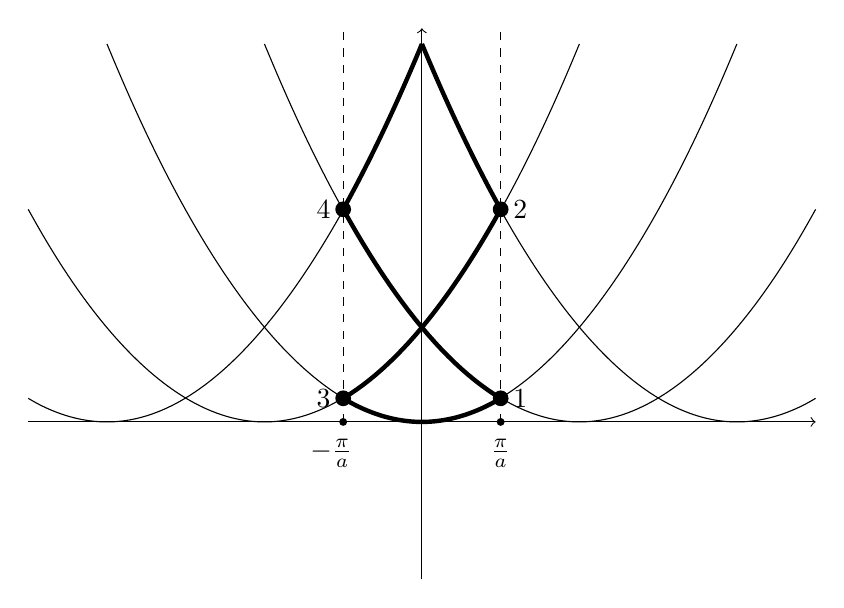
\begin{tikzpicture}[scale=1,auto=center]
			%\draw [help lines] (0,0) grid (2,2);
			\draw [->] (-5,0) -- (5,0);
			\draw [->] (0,-2) -- (0,5);
			\draw (-4,0.3*4^2) parabola bend (0,0) (4, 0.3*4^2);
			\draw (-2,0.3*4^2) parabola bend (2,0) (5, 0.3*3^2);
			\draw (-5,0.3*3^2) parabola bend (-2,0) (2, 0.3*4^2);
			
			\draw (0,0.3*4^2) parabola bend (4,0) (5, 0.3*1^2);
			\draw (-5,0.3*1^2) parabola bend (-4,0) (0, 0.3*4^2);
			\draw[domain=-1:1, ultra thick] plot (\x,{0.3*(\x)^2+1.2*\x+1.2});
			\draw[domain=-1:1, ultra thick]  plot (\x,{0.3*(-\x)^2+1.2*(-\x)+1.2} );
			\draw[domain=-1:0, ultra thick]  plot (\x,{0.3*(\x+2)^2+1.2*(\x+2)+1.2} );
			\draw[domain=0:1, ultra thick]  plot (\x,{0.3*((-\x)+2)^2+1.2*((-\x)+2)+1.2} );

			\draw[ultra thick] (-1,0.3) parabola bend (0,0) (1,0.3);
			\draw[ultra thick] parabola (-1,0.3) (1,9*0.3);	


			\node[fill,thick,circle, inner sep=0pt, minimum size=0.2cm] at (1,0.3)  {};
			\node[fill,thick,circle, inner sep=0pt, minimum size=0.2cm] at (1,9*0.3)  {};
			\node[fill,thick,circle, inner sep=0pt, minimum size=0.2cm] at (-1,0.3)  {};
			\node[fill,thick,circle, inner sep=0pt, minimum size=0.2cm] at (-1,9*0.3)  {};



			\node[] at (1.25,0.3)  {$1$};
			\node[] at (1.25,9*0.3)  {$2$};
			\node[] at (-1.25,0.3)  {$3$};
			\node[] at (-1.25,9*0.3)  {$4$};

			\node[fill,thick,circle, inner sep=0pt, minimum size=0.1cm] at (1,-0) {};
			\node[fill,thick,circle, inner sep=0pt, minimum size=0.1cm] at (-1,0)  {};
			\node[] at (1,-0.4) {$\frac{\pi}{a}$};
			\node[] at (-1.15,-0.4)  {$-\frac{\pi}{a}$};

			\draw[dashed] (-1,0) -- (-1,5);
			\draw[dashed] (1,0) -- (1,5);
		\end{tikzpicture}
	}
	\caption{Ritratto in fase dei momenti di particella libera}
	\label{Part:Lib}
\end{figure}
In Fig.\ref{Part:Lib}, è ben visibile che non vi è separazione tra le bande. \`E possibile passare in modo continuo da una banda all'altra nei punto in cui il vettore d'onda interseca la zona di Brillouin. in questo modo i punti $1,2,3,4$ hanno livelli quasi-degeneri, con energie di bande diverse che risultano molto vicine per lo stesso valore di $\vet k$. Si può passare ora a studiare il modo in cui il potenziale debole $U_e$ agisce sui livelli energetici. Il potenziale è riferito ad un reticolo diretto con una sua certa periodicità, è possibile rappresentarlo in serie di Fourier rispetto ai vettori $\vet q$ del reticolo reciproco 
\newl{U_e(x) = \sum_q U_q e^{i{\vet q}\cdot {\vet x}}\,\,\,\,\,\,\,\, \left(q=\frac{2\pi}{a}m\right).}
Adottando la convenzione di fissare la scala delle energie sul valor medio del potenziale allora si ottiene che $U_0=0$. Questo semplifica in modo essenziale gli sviluppi perturbativi. Riscrivendo l'equazione di Schroedinger con il contributo del potenziale
\newl{\left[-\frac{\hbar^2}{2m_e}\nabla^2+U_e(x)\right]\psi(x)=E\psi(x).}
A questo punto è necessario fare alcune considerazioni sulla funzione d'onda: essa può essere rappresentata sul sistema o.n.c delle onde piane, con opportuni coefficienti $C_k\in\C$
\newl{\psi(x)=\sum_kC_ke^{ikx}.}
Inserendo la funzione d'onda nell'equazione di Schroedinger appena scritta si ottiene il seguente problema agli autovalori
\newl{\sum_k\left[-\frac{\hbar^2}{2m_e}(-k^2)C_ke^{ikx}\right]+\sum_{q,k}U_qC_ke^{i(q+k)x}=E\sum_kC_ke^{ikx}}.
Moltiplicando per $e^{ik'x}$ ed integrando, si ottiene il seguente sistema per i coefficienti $C_k$
\newl{\left(\frac{\hbar^2}{2m_e}k^2 -E\right)C_k + \sum_q U_qC_{k-q} =0.}
Dall'ultima scrittura è possibile notare che il termine di potenziale è responsabile dell'accoppiamento tra i vari coefficienti $C_k$ infatti mette in realazione ogni coefficiente relativo ad un vettore $\vet k$ ad suo rispettivo nelle altre zone di Brillouin (che differenziano appunto di un vettore $\vet q$). Dato che può essere rimappato tutto nella prima zona di Brillouin, questo vuol dire che il termine di potenziale aggiunge accoppiamento tra i vari termini dello sviluppo. Tra i vari $\vet k$ vettori della prima zona di Brillouin si immagini di fissarne uno. In corrispondenza si avranno autofunzioni e autovalori indicizzati $\vet k$. Le funzioni d'onda dovranno essere la sovrapposizione di tutte le onde piane che distano di un vettore $\vet q'$ perchè come detto prima tutto viene rimappato nella prima zona
\newl{\psi_k(x)=\sum_{q'}C_{k-q'}e^{i(k-q')x}.}
Si noti che la somma è solo sui $\vet q'$ quindi è possibile riscrivere la funzione d'onda come
\newl{\psi(x)=e^{ikx}\sum_{q'}C_{k-q'}e^{-iq'x} = e^{ikx}u_k(x),}
questa forma è la stessa indicata per funzioni d'onda di elettrone libero in un potenziale cristallino dal teorema di Bloch. Questo fatto, con una certa forzatura, è possibile interpretarlo comeun'ulteriore prova a favore del teorema di Bloch. Prendendo la funzione d'onda appena scritta e usandola nell'equazione di Schroedinger si ottiene
\newl{\sum_{q'}\left[\frac{\hbar^2}{2m_e}(k-q')^2C_{k-q'}e^{i(k-q')x}\right]+\sum_{q',q"}U_{q"}C_{k-q'}e^{i(q"+k-q')x}=E_k\sum_kC_{k-q'}e^{i(k-q')x}}
Sfruttando nuovamente l'ortonormalità delle onde piane e integrando su $q"$ si ottiene, per ogni valore di $\vet k$, un sistema di equazioni accoppiate
\newl{\left[\frac{\hbar^2}{2m_e}(k-q)^2 -E_k\right]C_{k-q} +\sum_{q'}U_{q'-q}C_{k-q'}=0}
che una volta risolto fornisce i livelli energetici e i coefficienti dello sviluppo in serie della funzione d'onda. Ponendo $U_q=0$ si ritorna al caso precedente di particella libera
\newl{E_k,q = E(k-q)=\frac{\hbar^2}{2m_e}(k-q)^2}.
In questo caso $\vet q$ rappresenta il numero quantico che identifica la banda. Se ${\vet k} \sim {\vet q} /2$ si è in una condizione quasi degenere. Per valori di $\vet k$ lontani da questi punti le bande sono ben separate, il problema è solo in prossimità di questi punti. Per il calcolo della correzione dell'energia per mezzo di un potenziale debole è necessario considerare i due casi in modo separato e non si può effettuare una trattazione perturbativa standard. \`E possibile verificare che nel caso degenere per le due bande $q$ e $q'$ si ha 
\newl{\boxed{\Delta E=\abs{E(k-q)-E(k-q')}  \ll U .}}
Essendo la correzione dell'energia proporzionale a $U$  è quindi molto più significativa del caso non degenere in cui $\Delta E\gg U$ e la correzione di energia è proporzionale a $U^2$ quindi totalmente trascurabile. Ha quindi senso studiare solo la correzione dell'energia per il caso degenere poichè solo in questo caso si prevedono modifiche consistenti ai livelli energetici.
Per due bande degeneri generiche $\vet q_1$ e $\vet q_2$, tenendo conto solo dei termini dominanti si ottiene il seguente sistema algebrico
\newl{\left[E-E_{k,q_1}\right]C_{k-q_1} = U_{q_2-q_1}C_{k-q_1} \nonumber\\
	\left[E-E_{k,q_2}\right]C_{k-q_2} = U_{q_1-q_2}C_{k-q_2}
}
Soluzioni non nulle per i coefficienti dello sviluppo della funzione d'onda si hanno se si annulla il determinante della matrice
\[ \left| \begin{array}{cc}
E-E_{k,q_1} & -U_{q_2-q_1}  \\
-U_{q_1-q_2} & E-E_{k-q_2} \end{array} \right|.\]
Risolvendo per $E$ e osservando che $U_{q_1-q_2} = U^*_{q_2-q_1}$ (a causa del fatto che il potenziale è una funzione reale), si ottiene la correzione all'energia
\newl{\boxed{E(k)=\frac{E_{k,q_1}+E_{k,q_2}}{2}\pm \frac{1}{2}\sqrt{(E_{k,q_1}-E_{k,q_2})^2 + 4\abs{U_{q_1-q_2}} ^2 }   }.}
Questo indica che intorno a $(q_1+q_2)/2$ i livelli energetici di elettrone libero sono molto vicini e diventa molto singificativo il contributo del termine di potenziale. I livelli si \textit{respingono} dando vita ad un \textbf{gap di energia}, ovvero ad una zona di energie proibita. Possiamo notare che le correzioni all'energia diventano quindi sensibili quando $\abs{k-q_1} ^2 = \abs{k-q_2} ^2$ cioè quando siamo in una zona di quasi degenerazione. Posso ridefinire ${\vet k'} = \vet k - \vet q_1$ e $\vet q = \vet q_1 - \vet q_2$ in questo modo posso riscrivere la condizione di quasi degenerazione come
\newl{\abs{\vet k'} = \abs{{\vet k} - {\vet q}} }
cioè 
\newl{\boxed{\Delta{\vet k} = {\vet q}}}
che è la condizione di diffrazione di Von Laue. Quindi si spiega il motivo per il quale le bande si aprono in prossimità di quei punti, gli elettroni non possono stare in quelle posizioni e vengono diffratti.
\subsection{Soluzione elettrone libero in un potenziale periodico}
Nel paragrafo precedente sono stati elencati una serie di riusltati sulla formazione dei gap energetici in corrispondenza dei punti di quasi degenerazione. E' stato possibile verificare che la correzione all'energia è sensibile solo in questi punti. Lontano dai punti di quasi degenerazione la correzione all'energia diventa di ordine $O(N^2)$ quindi totalmente trascurabile. Per completare il concetto viene presentata, in modo più formale, la correzione agli autovalori per un elettrone libero in un potenziale periodico debole. Si consideri un potenziale realistico del tipo
\newl{V(x)=\sum_n v(x-na).
\label{PER:POT}}
La prima osservazione che è possibile fare è che il teorema di Bloch ci permette di separare, per ogni valore di $k$, il problema in due parti indipendenti. Si inizi col sostituire nell'equazione di Schrodinger la funzione d'onda di elettrone libero data dal teorema di Bloch
\newl{\left[-\frac{\hbar^2}{2m_e}\nabla^2 +V(x)\right]e^{ikx}u_k(x) = Ee^{ikx}u_k(x),}
in questo modo otteniamo un'equazione per la parte periodica
\newl{\left[\frac{\hbar^2}{2m_e}\left(k^2-2ik\frac{d}{dx}-\frac{d^2}{dx^2}\right)+V(x)-E\right]u_k(x)=0}
che in generale ha un'infinita di soluzioni ortogonali tra loro e sono del tipo
\newl{\int_{-L/2}^{+L/2}dx\,u^*_{k,n}(x)u_{k-m}(x) = \delta_{nm}N\int_{-a/2}^{+a/2}dx\,u^*_{k,n}(x)u_{k',m}(x).}
L'integrale è condotto su tutto il cristallo sfruttando la periodicità della funzione $u_k(x)$. L'integrale da $-L/2$ a $+L/2$ è stato quindi ricondotto alla sola cella unitaria.
Questo fatto è di interesse perchè mostra come è fatta la soluzione per quel tipo di problema e mette in luce che per valori di $k$ diversi, le soluzioni sono ortogonali tra loro. Riprendiamo gli stessi conti per una funzione d'onda di Bloch e sommiamo sempre su tutti i $k$ del reticolo
\newl{\int_{-L/2}^{+L/2} \psi^*_{k,n}(x)\psi_{k',n}(x)\,dx &=& \int_{-L/2}^{+L/2} e^{i(k'-k)x}u^*_{k,n}(x)u_{k',n}(x)\,dx \\
&=& \left(\sum_p e^{ip(k'-k)a}\right)\int_{-a/2}^{+a/2}e^{i(k'-k)x}u^*_{k,n}(x)u_{k',n}(x)\,dx ,	\nonumber}
i vettori p sono su tutto il reticolo e l'integrale è diverso da zero solo se $k$ e $k'$ coincidono, in questo modo si ha che
\newl{\sum_p e^{ip(k'-k)a} = N\delta_{k,k'}.}
In effetti non si può dire nulla sull'ortogonalità delle parti periodiche per diversi valori di $k$. L'unica cosa che si può dire è che per lo stesso valore di $k$, stati d'onda  di Bloch sono ortogonali.\footnote{Molto oscuro...}
\subsection{Metodo delle onde piane}
Il problema dell'elettrone libero in un potenziale periodico è possibile trattarlo in modo numerico. Dato il potenziale periodico, un approccio particolarmente efficace è quello di usare una base di onde piane, in particolar modo se il potenziale è periodico. \`E possibile definire a priori la forma di queste onde piane. Possiamo sfruttare la periodicità del reticolo e il teorema di Bloch che fissato un $k$, forniscono una forma particolare di base di onde piane
\newl{b_{n,k}(x)=\frac{1}{\sqrt{L}}e^{i(k+G_n)x}\,\,\,\, , \,\,\,\,\,\,\,G_n=\frac{2\pi}{a}n 
\label{BASE:BLOCH}}
la giusta base deve essere quindi del tipo $\exp(ikx)$ come stati di Bloch con vettori di Bloch $k$. Per un potenziale periodico come quello in formula \ref{PER:POT} abbiamo che la trasformata di Fourier è data da
\newl{\tilde{V}(G)=\frac{1}{L}\int_{-L/2}^{+L/2}V(x)e^{iGx}dx = \frac{1}{L}\left( \sum_p e^{ipGa} \right)\int_{-a/2}^{+a/2}v(x)e^{-iGx}dx }
e i vari componenti sono diversi da zero solo per un discreto insieme di vettori $G$, infatti il fattore $\sum_pe^{ipGa}$ è zero eccetto quando $Ga$ è un multiplo di $2\pi$, dove i $G_n$ sono quelli definiti in \ref{BASE:BLOCH}. In questo modo è possibile trovare
\newl{\tilde{V}(G)=\frac{1}{a}\int_{-a/2}^{+a/2} v(x) e^{-iG_nx}dx.}
L'integrale è calcolato per un singolo termine nel potenziale e in una singola cella unitaria. Al limite termodinamico, quindi per $N\to\infty$ questa cosa è ben definita.

\subsection{Legame Forte - Tight Binding}
Bho...

\subsection{Alcune considerazioni di carattere generale}
Risolvendo il problema degli elettroni liberi in potenziale periodico cristallino è stato possibile studiare il modo in cui si vengono a formare le bande di energia all'interno di un cristallo e e gli stati assunti dagli eletroni. In questo paragrafo si vuole mettere in risalto l'importanza di tutti i concetti precedentemente presentati e collegarli insieme per capire il modo in cui effettivamemente vengono usati in fisica. L'obiettivo principale è sempre quello di essere in grado, attraverso opportuni esperimenti, di determinare la struttura cristallina e le proprietà quantistiche del materiale in studio. Come visto precedentemente, il reticolo cristallino può essere ricostruito tramite diffrazione di Von Laue. Il teorema di Bloch, insieme alla soluzione del modello di elettrone libero in potenziale debole periodico, aggiunge l'informazione che i punti di diffrazione, trovati con la legge di Von Laue, sono punti di quasi-degenerazione per l'energia in cui l'elettrone potrebbe, in modo continuo, passare da una banda all'altra. Inserendo in modo perturbativo il contributo del potenziale è stato possibile vedere che si vengono a creare delle zone di energie non permesse. Quello che ci può dare un'idea concrete della forma della banda sono le superfici ad energia costante. Consideriamo quelle zone in cui il gradiente dell'energia è nullo e andaimo a studiarne la geometria
\newl{\nabla E(k) =0 \implicaa \frac{\hbar^2}{2m_e}\left(k^2-\left(\frac{q_1+q_2}{2}\right)^2\right)=0}
che è nulla in 
\newl{\boxed{k=\frac{q_1+q_2}{2}}.}
Questi valori di $k$ sono quelli che delimitano la Prima zona di Brillouin, quindi le superfici ad energia costante raggiungono la prima zona di brillouin con $\nabla E =0$ cioè sono normali alla superficie della zona.
\subsection{Proprietà vibrazionali dei solidi}
Nella sezione precedente ci si è concentrati sulla dinamica degli elettroni, visti come pacchetti d'onda che si muovono in un potenziale periodico. L'attenzione ora verrà spostata alle proprietà vibrazionali del reticolo. Il sistema cristallino viene sempre considerato con la solita approssimazione adiabatica. Elettroni e nuclei hanno scale di tempo di evoluzioni molto diverse quindi possiamo sempre separare lo studio delle due componenti, appunto moto degli elettroni e moto dei nuclei. L'Hamiltoniana del sistema da studiare è
\newl{-\frac{\hbar^2}{2}\left(\sum_i\frac{\nabla^2_{R_i}}{M_i}\right)\psi(R) + U_{\text{ad.}}(R) \psi(R) - E\psi(R) = 0.}
Dove con $i, j$ si identifica l'indice di particella, mentre con le lettere greche $\alpha, \beta$ si indentifica l'indice di direzione.
Supponiamo che $\vet R_0$ sia il punto di equilibrio di sistema, in questo caso posso sviluppare il potenziale adiabiatico in un intorno di $\vet R_0$ 
\newl{U_{\text{ad.}} =U_0 +  \sum_{i,\alpha,j,\beta} \left(\frac{\partial^2 U_{\text{ad.}}}{\partial u_{i,\alpha} \partial u_{j,\beta}}\right)_{R_0} u_{i,\alpha} u_{j,\beta} = U_0 + \Phi_{i,\alpha, j, \beta} u_{i,\alpha} u_{ j,\beta}  }
La $\vet \Phi$ è chiamata \textit{Matrice delle costanti di Forza} e rappresenta l'approssimazione parabolica del potenziale adiabatico lungo le varie direzioni, quindi le forze di richiamo, in approssimazione quadrata, lungo i vari assi. Per scrivere l'equazione del moto dei nuclei si passa dalla lagrangiana del sistema in cui i vari nuclei sono legati da una forza di richiamo, lungo le varie direzioni, indicata dalla matrice delle costanti di forza $\vet \Phi$. Se il numero di particelle è $N$ avrò $3N$ equazioni 
\newl{\mathcal{L}= \frac{1}{2}M_i(\dersf{u} _{i,\alpha})^2 - \frac{1}{2}  \Phi_{i,\alpha, j, \beta} u_{i,\alpha} u_{ j,\beta} }
per comodità di notazione sostituisco $q_{i,\alpha} = u_{i,\alpha}$ in questo modo posso scrivere le equazioni di Lagrange nella solita forma
\newl{\frac{d}{dt}\frac{\partial \mathcal{L}}{\partial \dersf{q} } - \frac{\partial \mathcal{L}}{\partial q}=0 }
derivando si ottengono le equazioni del moto
\newl{M_i \derrsf{u} _{i,\alpha}  + \Phi_{i,\alpha, j,\beta}u_{j,\beta} =0 .}
Nella prima parte, la ripetizione dell'indice $i$ nella matrice delle masse e nella parte di velocità non è da intendersi come somma covariante, in realtà $i$ è un indice libero che non si somma. Risolvo l'equazione differenziale nello spazio $\vet k$, passo quindi alla trasformata di Fourier 
\newl{k^2 {\vet M} u(k)  - {\vet \Phi} u(k) = 0.}
Definisco per semplicità $w = \sqrt{{\vet M}} u$, ottenendo
\newl{k^2 w - \left(\sqrt{{\vet M}}\right)^{-1} {\vet \Phi} \left(\sqrt{{\vet M}}\right) w =0 .}
La matrice ${\vet D} = \left(\sqrt{{\vet M}}\right)^{-1} {\vet \Phi} \left(\sqrt{{\vet M}}\right)$ è comunemente conosciuta col nome \textit{Matrice Dinamica}. Non è necessariamente diagonale quindi si trova un  operatore che sia in grado di diagonalizzarla. Si supponga che esista un operatore identificato dalla matrice $\vet S$ che goda delle seguenti proprietà
\newl{{\vet S}^\dagger {\vet S} = {\vet 1}, \text{e renda diagonale: }  {\vet S}^\dagger {\vet D} {\vet S} = 
	\left(\begin{array}{c c c}
		w_1^2&  &  \\
		 & \ddots &  \\
		 &  & w_N^2 \end{array}\right)
.}
Le coordinate degli autovettori di ${\vet D}$ sono
\newl{q={\vet S}^\dagger w \implicaa q = {\vet S}^\dagger {\vet M} ^{\frac{1}{2}} u \implicaa u = {\vet M}^{-\frac{1}{2}} {\vet S} q.}
Riscrivo la lagrangiana nella nuova base diagnonale
\newl{\mathcal{L} = \frac{1}{2} \dersf{w} ^\dagger \dersf{w} -\frac{1}{2} w^\dagger {\vet D} w = \frac{1}{2} \dersf{q} {\vet S^\dagger} {\vet S}\dersf{q} -\frac{1}{2} q {\vet S}^\dagger {\vet D}  {\vet S} q  ,}
essendo tutto diagonale posso scrivere la Lagrangiana in funzione di un singono indice
\newl{\sum_\gamma \mathcal{L}_\gamma = \frac{1}{2} \sum_\gamma \left[ \left(\dersf{q} _\gamma\right)^2 -k^2_\gamma q_\gamma\right].}
Effettuando il cambio di variabili $Q_\gamma = \sqrt{w_\gamma} q_\gamma$ ottengo
\newl{\mathcal{L} = \frac{1}{2}\sum_i \left[\frac{\dersf{Q} _i^2}{w_i}-w_iQ_i^2\right],}
che è praticamente la lagrangiana di un oscillatore armonico, infatti tramaite trasformata di Legendre arrivo quasi alla tipica Hamiltonina di un oscillatore armonico
\newl{H = \sum_i w_i \left(\frac{\op{P_i} ^2 + \op{Q_i} ^2}{2}\right)}
che, per come è stato impostato il problema,  è un risultato abbastanza aspettato. Usando gli operatori di salita e discesa\footnote{che sono definiti come: $\op{a} _i^\dagger =\frac{1}{\sqrt{2\hbar}} \left(\op{Q} _i - i\op{P} _i\right)$ e $\op{a} _i = \frac{1}{\sqrt{2\hbar}} \left(\op{Q} _i + i \op{P} _i\right)  $. }  arrivo esattamente all'Hamiltoniana di un oscillatore
\newl{H=\sum_i\hbar w_i \left(\op{a} _i^\dagger \op{a} _i +\frac{1}{2}\right).}
Quanto scritto vale per un sistema di $N$ atomi senza tener conto della periodicità del reticolo. Introducendo il fatto che il sistema è periodico con periodicità quella del reticolo, per la matrice delle costanti di forza vale la seguente scrittura
\newl{\phi_{i,n\alpha, j,n'\beta} = \phi_{i,(n'+n")\alpha, j,(n'+n")\beta} .}
Data la periodicità del sistema posso scrivere gli stati come stati di Bloch costituiti quindi da una parte periodica, con periodicità del reticolo, e da una parte di onda piana. Nello spazio di Fourier lo stato di block è
\newl{
	&&\tildato{W} _{i,n\alpha} = \sqrt{M_i} u_{i,n\alpha}\nonumber\\
	&&u_{i,n\alpha} = \frac{\tildato{W} _{i,n\alpha}}{\sqrt{M_i}} =  \frac{W_{i,n\alpha}}{\sqrt{M_i}} e^{ikR}
}
Sostituendo gli stati di Bloch nella Lagrangiana, tramite le equazioni di E-L arrivo ancora all'equazione del moto nello spazio $k$
\newl{
	&&k^2{\vet M} u -{\vet \Phi}u =0\nonumber\\
	&&k^2M_i\frac{W_{i,n\alpha}}{\sqrt{M_i}} e^{ikR_n} - \Phi_{i,n\alpha,j,n'\beta} \frac{W_{i,n\alpha}}{\sqrt{M_i}} e^{ikR_n}=0 
}
che usando la periodicità può essere riarrangiata in una forma più evidente
\newl{ \left(k^2W_{i,\alpha}({\vet k})  - \Phi_{i,\alpha,j,(n'-n)\beta} \frac{W_{j,(n'-n)\beta}({\vet k})}{\sqrt{M_j M_i}}\right) e^{ikR_n}=0  }
\subsection{Reticolo monodimensionale a due atomi}
Un esempio applicativo di quanto detto fin'ora è rappresentato dal reticolo monodimensionale con due specie atomiche.

\begin{center}
	\fbox{
		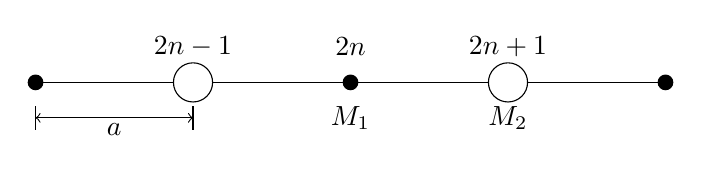
\begin{tikzpicture}[scale=1,auto=center]
			\draw (0,0) -- (1.75,0);
			\node[fill,thick,circle, inner sep=0pt, minimum size=0.2cm] at (0,0)  {};
			\node[draw, circle, inner sep=5pt, minimum size=0.1cm] at (2,0) {};
			\draw (2.25,0) -- (4,0);
			\node[fill,thick,circle, inner sep=0pt, minimum size=0.2cm] at (4,0)  {};
			\draw (4,0) -- (5.75,0);
			\node[draw, circle, inner sep=5pt, minimum size=0.1cm] at (6,0) {};
			\draw (6.25,0) -- (8,0);
			\node[fill,thick,circle, inner sep=0pt, minimum size=0.2cm] at (8,0)  {};


			\node[] at (2,0.45) {$2n-1$};
			\node[] at (4,0.45) {$2n$};
			\node[] at (6,0.45) {$2n+1$};
			\node[] at (4,-0.45) {$M_1$};
			\node[] at (6,-0.45) {$M_2$};

 			\draw (0,-0.3) -- (0,-0.6);
			\draw (2,-0.3) -- (2,-0.6);
			\draw[<->] (0,-0.45) -- (2,-0.45);
			\node[] at (1,-0.6) {$a$};


		\end{tikzpicture}
	}
\end{center}
I due atomi sono rappresentati dalle due diverse masse $M_1$ e $M_2$. La cella reticolare è di dimensione $2a$. Il fatto che siano presenti due tipi diversi di atomi questo permette di scrivere due equazioni del moto 
\newl{
	&&M_1 \frac{d^2u_{2n+1}}{dt^2} = -\alpha(2u_{2_n+1}-u_{2_n}-u_{2_n+2} )\\
	&&M_2 \frac{d^2u_{2n+2}}{dt^2} = -\alpha(2u_{2_n+2}-u_{2_n+1}-u_{2_n+3})
}
Dove $\alpha$ è la costante di accoppiamento interatomica, $n$ è un indice intero e scorre su tutti gli atomi di tipo $M_1$ quando è dispari e $M_2$ quando è pari. Le equazioni scritte sopra sono palesemente accoppiate. Abbiamo un totale di $2N$ equazioni differenziali accoppiate, da risolvere simultaneamente. Per risolvere questo tipo di equazioni si prende sempre in cosiderazione il sistema in studio e si formula un'Ansazt. Quella più attendibile è 
\newl{\left[\begin{array}{c}
		u_{2n+1} \\
		u_{2n}
\end{array}\right] = 
\left[\begin{array}{c}
	A_1e^{iqX_{2n+1}} \\
	A_2e^{iqX_{2n+2}}
\end{array}\right] e^{-i\omega t} .
}
In questo modo tutti gli atomi di massa $M_1$ hanno tutti ampiezza $A_1$ e lo stesso vale per gli atomi di massa $M_2$ che hanno ampiezza $A_2$. Sostituendo la soluzione del sistema di equazioni differenziali accoppiate scritto inizialmente, passando attraverso alcune drastiche semplificazioni si arriva alla semplice scrittura
\newl{\left(\begin{array}{cc}
		2\alpha - M_1\omega^2 & -2\alpha \cos(qa) \\
		-2\cos(qa) & 2\alpha -M_2\omega^2
	\end{array}\right) 
	\left(\begin{array}{c}
			A_1\\
			A_2
	\end{array}\right) = 0,
}
che è l'equivalente di due equazioni differenziali simulatanee nelle variabili $A_1$ e $A_2$. Le equazioni sono omogenee e hanno soluzione non banale solo se il determinante si annulla. La condizione diventa quindi
\newl{\text{det} \left|\begin{array}{cc}
	2\alpha - M_1\omega^2 & -2\alpha \cos(qa) \\
	-2\cos(qa) & 2\alpha -M_2\omega^2
	\end{array}\right| = 0.
}
A questa condizione corrisponde un'equazione nella variabile $\omega^2$ le cui soluzioni sono
\newl{\omega^2 =\alpha\left(\frac{1}{M_1} + \frac{1}{M_2}\right)\pm\alpha\sqrt{\left(\frac{1}{M_1} + \frac{1}{M_2} \right)^2 - \frac{4\sin^2(qa)}{M_1M_2}} .}
Come è possibile notare in Fig.~$\ref{PH:AC}$, in corrispondenza dei due diversi segni si distinguono due \textit{branches}, ottici e acustici.
\begin{figure}
	\centering
	\fbox{
		\begin{tikzpicture}[scale=1,auto=center]
			\draw[->] (0,0) -- (0,5);
			\draw[->] (-2.5,0) -- (2.5,0);
			\node[] at (0,5.3) {$\omega$};
			\node[] at (0,-0.25) {$0$};
			\node[] at (2,-0.25) {$\pi/2a$};
			\node[] at (-2,-0.25) {$-\pi/2a$};
			\draw[dashed] (2,0) -- (2,5);
			\draw[dashed] (-2,0) -- (-2,5);
			\draw[domain=-2:2] plot (\x,{3*sqrt((sin(\x*45))^2) });
			\draw[domain=-2:2] plot (\x,{3*sqrt((sin((\x+4.5)*20))^2)+1});
			
		\end{tikzpicture}
	}
	\caption{Fononi: bande acustiche e bande ottiche}
	\label{PH:AC}
\end{figure}
I rami acustici partono da $(0,0)$ e sono funzione crescente di $q$. Intorno a zero il comportamento è in prima approssimazione lineare, il che torna con le relazioni di dispersione lineare del suono nei mezzi, ben conosciuti in fisica calssica, la curva poi satura sui bordi della zona di Brillouin. Il ramo ottico invece, per $q=0$ vale 
\newl{\omega = \left[2\alpha\left(\frac{1}{M_1}+\frac{1}{M_2}\right)\right]^{1/2}} 
e descresce molto lentamente nell'avvicinarsi al bordo della zona di Brillouin. La frequenza di questo braccio non varia in modo apprezzabile lungo tutto il range di valori di $q$, infatti solitamente si considera costante. Il range di frequenze, tra la parte alta del ramo acustico e la parte bassa del ramo ottico, rappresenta una zona di frequenze non consentite. In questo range il cristallo non può trasmettere nessun tipo di onda. Il risultato che si ha è quello che ogni onda di frequenza proibita, che interagisce col cristallo, viene fortemente attenuata.
